\documentclass[12pt]{article}
\usepackage[margin=1in]{geometry}
\usepackage{times}
\usepackage{graphicx}
\usepackage{float}
\usepackage{caption}
\usepackage{subcaption}
\usepackage{lineno}
\usepackage{amsmath}
%\usepackage{natbib,hyperref}
\linenumbers

\newcommand*{\met}{\ensuremath{E_\text{T}^\text{miss}}}

\author{Danika MacDonell}
\title{Search for Dark Matter Production in As}
\begin{document}
\maketitle

\section{Introduction}

The proposed thesis is a search for dark matter production at the LHC, in association with a higgs boson $s$ in the dark sector decaying to W bosons in the ATLAS detector. The search is motivated and optimized with a signal model in which the $s$ is produced in association with a new Z' gauge boson, which decays to a pair of massive dark matter particles. 

As the dark matter produced is not expected to interact to any measurable extent with the normal matter constituting the ATLAS detector, the momentum that it carries will escape undetected. As such, momentum conservation in the plane transverse to the beam line implies that the signal will exhibit a signature of high missing momentum in the plane transverse to the beam line (\met) in the final state. 

The aim of the analysis is to apply selections to data from the ATLAS detector to optimize the sensitivity of the data to the dark Higgs signal model, and then compare the data with the sum of Monte Carlo simulated standard model background and signal processes to search for an excess consistent with signal+background. 

The search is split into two separate analyses:

\begin{enumerate}

\item \textbf{The hadronic decay channel:} Each of the two W bosons produced from the $s$ decay to quarks, which subsequently hadronize in the detector, and are measured as localized energy deposits called jets in the calorimeter system.

\begin{equation}
\nonumber
WW \rightarrow q\bar{q}+q\bar{q}
\end{equation}

Given the branching fraction of 0.68 \cite{PDG} for $W \rightarrow qq$ decay, the fully hadronic WW decay occurs with a branching fraction of 0.46 ($0.68^2$). This channel has the advantage of being able to fully reconstruct the momenta of both W bosons, and as such the $s$ mass. The drawback is that there are standard model processes which also produce a final state of multiple jets in the detector with large production cross section, a subset of which pass the other signal selection criteria and represent a sizeable background in the analysis. 

\item \textbf{The semileptonic decay channel:} One W boson decays to quarks which hadronize to jets, and the other decays to a lepton and a neutrino, where the lepton is either an electron or a muon. 

\begin{equation}
\nonumber
WW \rightarrow q\bar{q}+\ell\nu
\end{equation}

Despite its lower branching fraction of 0.29 \cite{PDG} compared with the fully hadronic decay channel, the semileptonic channel has the advantage that the requirement of having one lepton in the final state reduces the background of standard model processes. However, this comes at the cost of additional \met from the neutrino production, which both inhibits reconstruction of the leptonically-decaying W boson and mimics the \met associated with dark matter production in the signal model. The proposed 

\item \textbf{The fully leptonic decay channel:} Both W bosons decay to a lepton and a neutrino. This channel would give a clean signature of two leptons and no jets, but is currently not considered as a worthwhile search channel due to its relatively low branching fraction of 0.046 \cite{PDG}.

There is an ongoing analysis searching for the dark Higgs signal in the hadronic decay channel, and the proposed thesis will focus on the semileptonic decay channel. 

\end{enumerate}

In the event that no above-background excess is observed, the search will be able to exclude at some level of statistical confidence - typically 95\% - a range of  Z' and $s$ masses that would have been observed if the signal under consideration actually occurred in nature. Assuming the search in the hadronic decay channel also fails to find any excess, the two channels will be statistically combined to obtained overall exclusion limits on the Z' and $s$ masses for both searches. 

\section{Motivation}

The proposed thesis work would contribute to the extensive ongoing dark matter search program at the LHC. This search program is motivated by compelling evidence from observational astronomy for the existence of dark matter constituting 85\% \cite{planck} of all matter in the universe. Despite clear evidence from observational astronomy for its gravitational interactions with normal matter, dark matter has yet to be detected through the weak, strong or electromagnetic interactions. As such, its composition and non-gravitational interactions - if any - remain largely a mystery. However, there is strong evidence to suggest that dark matter could be comprised of fundamental particles, and there are no particles in the standard model of particle physics that could represent viable dark matter candidates \cite{feng}. Dark matter is therefore typically assumed to be a ``beyond-standard-model" (BSM) particle. 

\subsection{Dark Matter Search Methods}
There are three complementary approaches used to search for particle dark matter: direct and indirect detection, and collider searches. Direct detection searches \cite{Schumann_2019, 2015gya} aim to directly detect evidence of a recoil induced by elastic scattering between a dark matter in the galactic halo passing through the detector and a target particle in the detector. Indirect searches \cite{CIRELLI_2012, conrad} use observational data to search for evidence of products produced by dark matter annihilation or decay in particular regions of the observable universe expected to have a high dark matter density. Collider searches \cite{DM_colliders} such as the proposed thesis work study the decay products from high-energy collisions of subatomic particles to search for an excess of events above the background of standard model processes that could be consistent with signatures of dark matter production in models of physics beyond the standard model.

\subsection{Models of Dark Matter Production at Colliders}
Models of dark matter production in colliders can range in complexity from an effective field theory, where the dark matter production mechanism is completely unspecified, to a complete model such as supersymmetry \cite{susy_dm} which predicts viable matter candidates as part of a hypothesized extension to the standard model designed to address other phenomena unexplained by the standard model. 

The effective field theory approach treats the annihilation of colliding partons into dark matter as a contact interaction, with the production rate determined by a single parameter \cite{DM_colliders}. As long as a measurable standard model particle is also produced in the interaction (eg. a gluon radiating off one of the colliding quarks, see figure \ref{fig:eft_simplified_model}), the EFT framework can be applied to any mono-X signature at the LHC, where a standard model particle X is measured along with missing transverse momentum in the detector. This makes the framework generally usable in terms of providing a motivation for and theoretical framework with which to interpret a range of generic search channels that can be readily selected for in LHC collision data. However, the EFT framework relies on the assumption that the the mediator(s) of the interaction is (are) much more massive than the energy transfer in the interaction \cite{DM_colliders, beyond_eft}. If this assumption is inaccurate, the EFT framework becomes invalid, and a more complete model is needed to specify additional details of the process leading to dark matter pair production. 

\begin{figure}[H]
	\centering
	\begin{minipage}[b]{0.45\textwidth}
	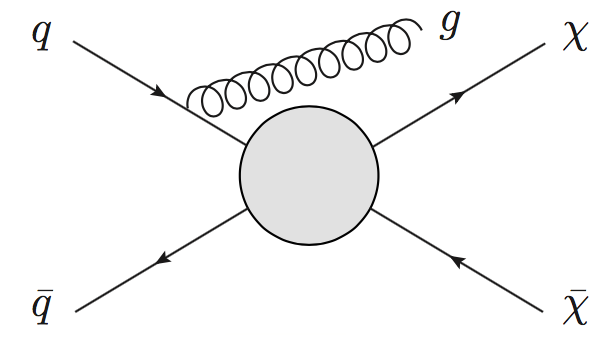
\includegraphics[width=0.9\textwidth]{figures/EFT_Signature.png}
	\end{minipage}
	\begin{minipage}[b]{0.45\textwidth}
	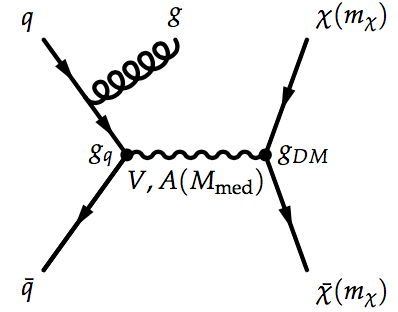
\includegraphics[width=0.8\textwidth]{figures/simplified_model.png}
	\end{minipage}
	\caption{Left: Mono-jet process in the EFT framework (source: \cite{beyond_eft}). Right: Mono-jet process in a simplified model framework, where the pair production of dark matter occurs via a vector or axial-vector mediator (source: \cite{dm_forum})}
	\label{fig:eft_simplified_model}
\end{figure}

In principle, complete theories of physics beyond the standard model, such as the minimal supersymmetric standard model (MSSM) \cite{mssm} can offer theoretically motivated and experimentally accessible models which specify the details of candidate processes by which the colliding partons may annihilate to produce dark matter. However, these theories tend to be quite complex, with many free parameters - over 100 in the case of MSSM \cite{DM_colliders} - most of which need to be fixed to for a reasonably testable model. Relying on complete theories alone to guide experimental signatures may run the risk of missing important parameter space of new physics for which a complete theory has not yet been developed. 

Simplified models, widely used in recent and ongoing dark matter searches at the LHC, are designed to bridge the gap between EFT and complete theories. They provide a `first-order' description of theoretically motivated new physics scenarios that could be accessible at collider energies. They provide guidance for experimental searches for new physics without fully specifying the details of any additional new physics at energies above the collider scale that would be needed for a complete theory \cite{DM_colliders}. In terms of dark matter production at the LHC, one or more new mediators associated with new physics scenarios may be considered which allow for mixing between standard model particles and dark matter. The process by which the mixing occurs is represented with a tree-level diagram whose experimental signature would be accessible at LHC energies, such as the diagram shown in figure \ref{fig:eft_simplified_model}, included as a dark matter benchmark model in the 2015 report of the ATLAS/CMS Dark Matter Forum \cite{dm_forum}. The proposed thesis will investigate an experimental signature of dark matter production at the LHC that is motivated by the simplified model involving a higgs boson in the dark sector described in Section 2.3 below. 

\subsection{Theory}

\begin{figure}[H]
	\centering
	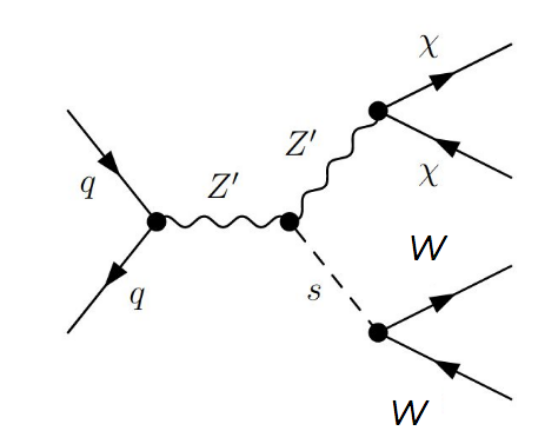
\includegraphics[width=0.4\textwidth]{figures/Signal.png}
	\caption{Signal model}
	\label{fig:signal}
\end{figure}

\subsection{Experimental Background}
\subsubsection{Re-interpretation of mono-H(bb) search for dark higgs mediator}
\begin{figure}[H]
	\centering
	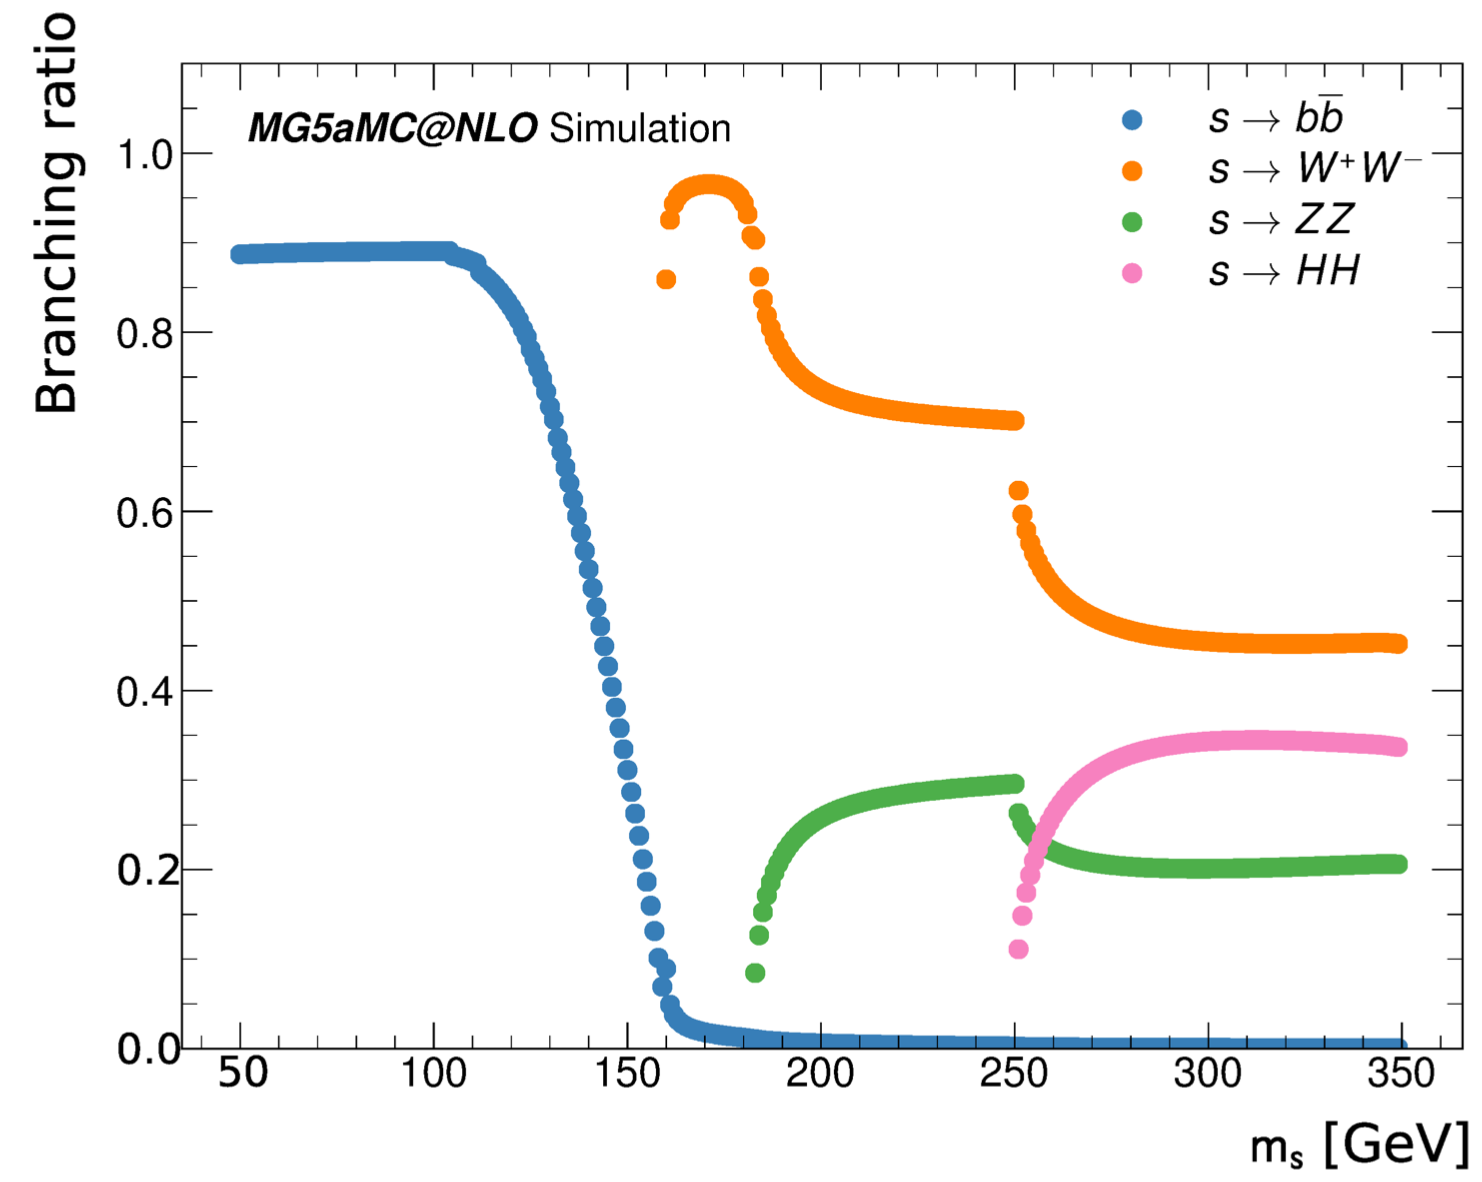
\includegraphics[width=0.7\textwidth]{figures/BR_vs_mass.png}
	\caption{Higgs decay branching ratios as a function of Higgs boson mass}
	\label{fig:higgsbrs}
\end{figure}
\begin{figure}[H]
	\centering
	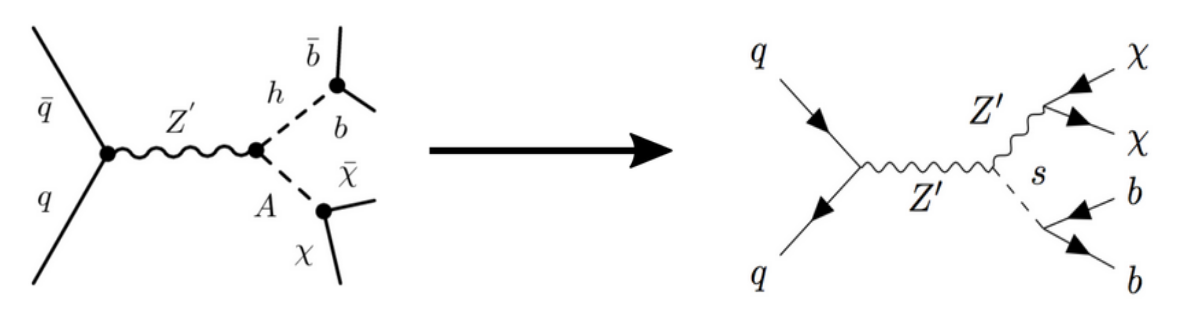
\includegraphics[width=0.9\textwidth]{figures/monohbb_reinterpretation.png}
	\caption{Re-interpretation of mono-H(bb) search using dark higgs boson with floating mass}
	\label{fig:monohbbreinterp}
\end{figure}

\section{Brief intro to LHC and ATLAS detector}
\begin{figure}[H]
	\centering
	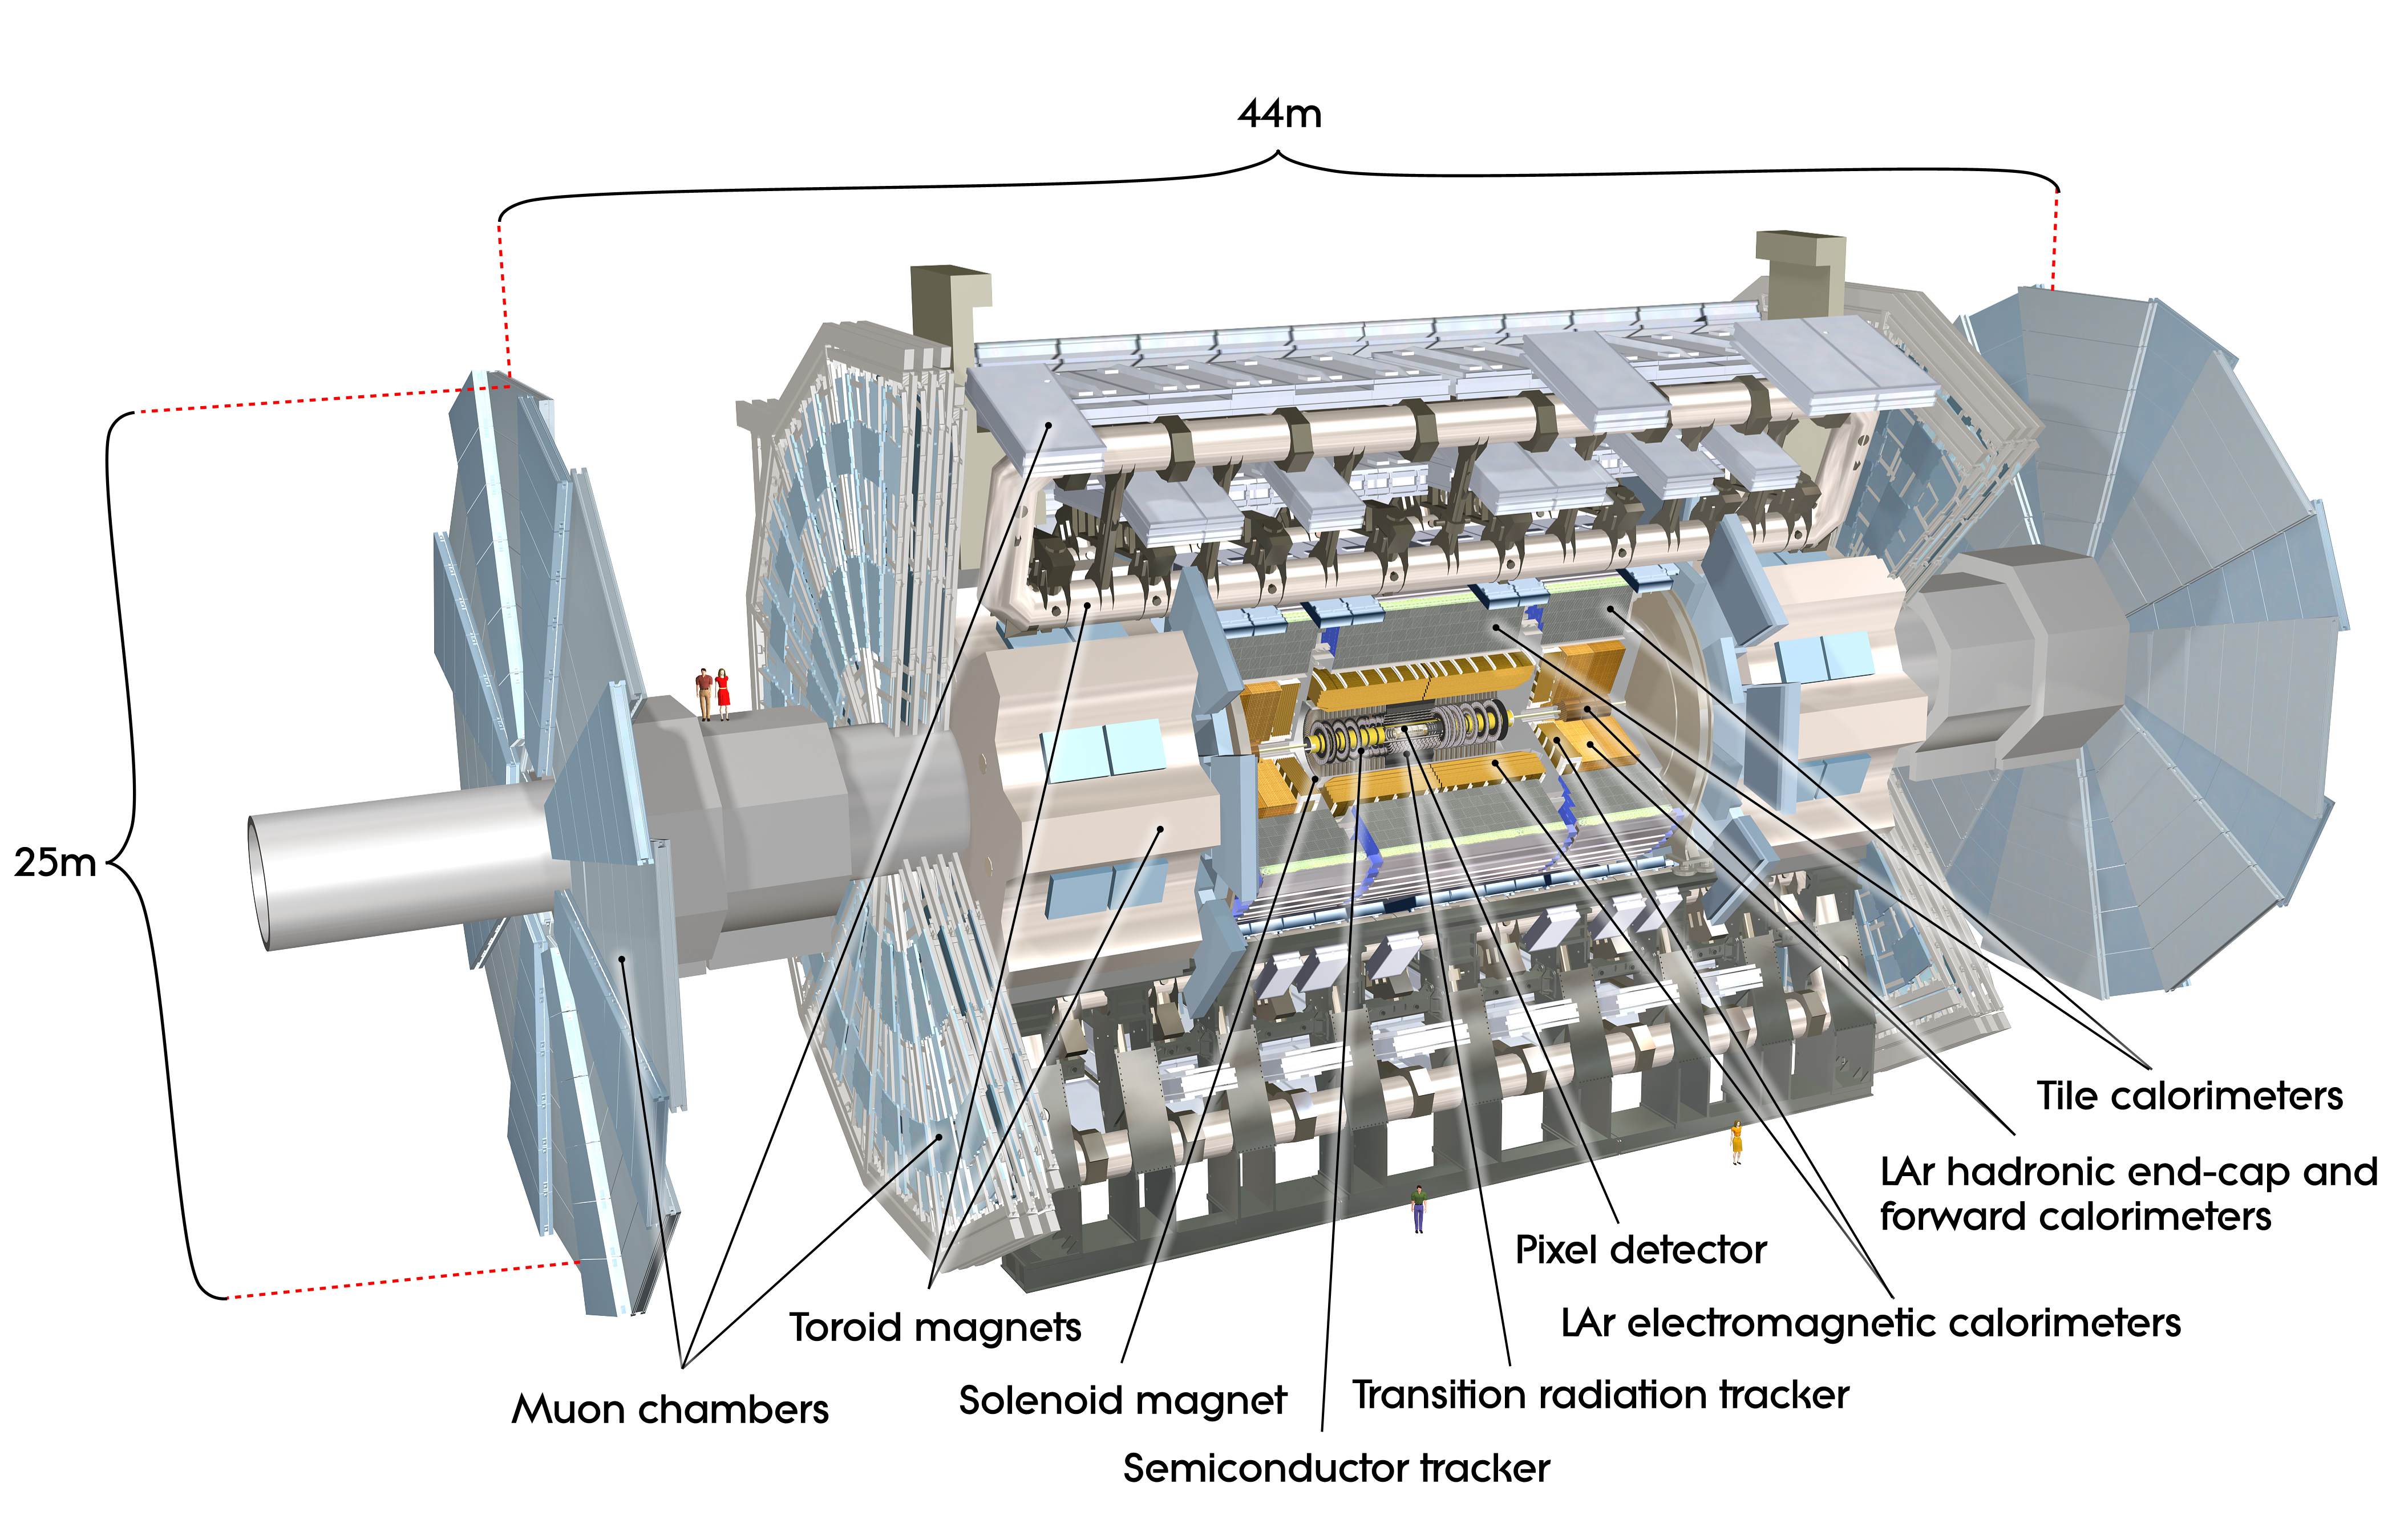
\includegraphics[width=0.85\textwidth]{figures/detector.jpg}
	\caption{ATLAS detector}
	\label{fig:detector}
\end{figure}
\begin{itemize}
\item Inner detector
\item EM cal
\item Had cal
\item Muon spectrometer
\end{itemize}

\section{Ongoing analysis of mono-s(WW) hadronic channel}
\begin{itemize}
\item Preselection
\item Signal region selection
\item Control regions
\item Very brief summary of systematics (exp and modeling)
\item Sensitivity estimates
\item RECAST
\end{itemize}

\section{Signal Sample Generation for Semileptonic Channel}

The mass of a dark matter particle is fixed to 200 GeV/c$^2$, and the Z' and dark higgs masses are allowed to vary from 500 GeV/c$^2$ to 2500 GeV/c$^2$ and 160 GeV/c$^2$ to 360 GeV/c$^2$, respectively. 

\begin{figure}[H]
	\centering
	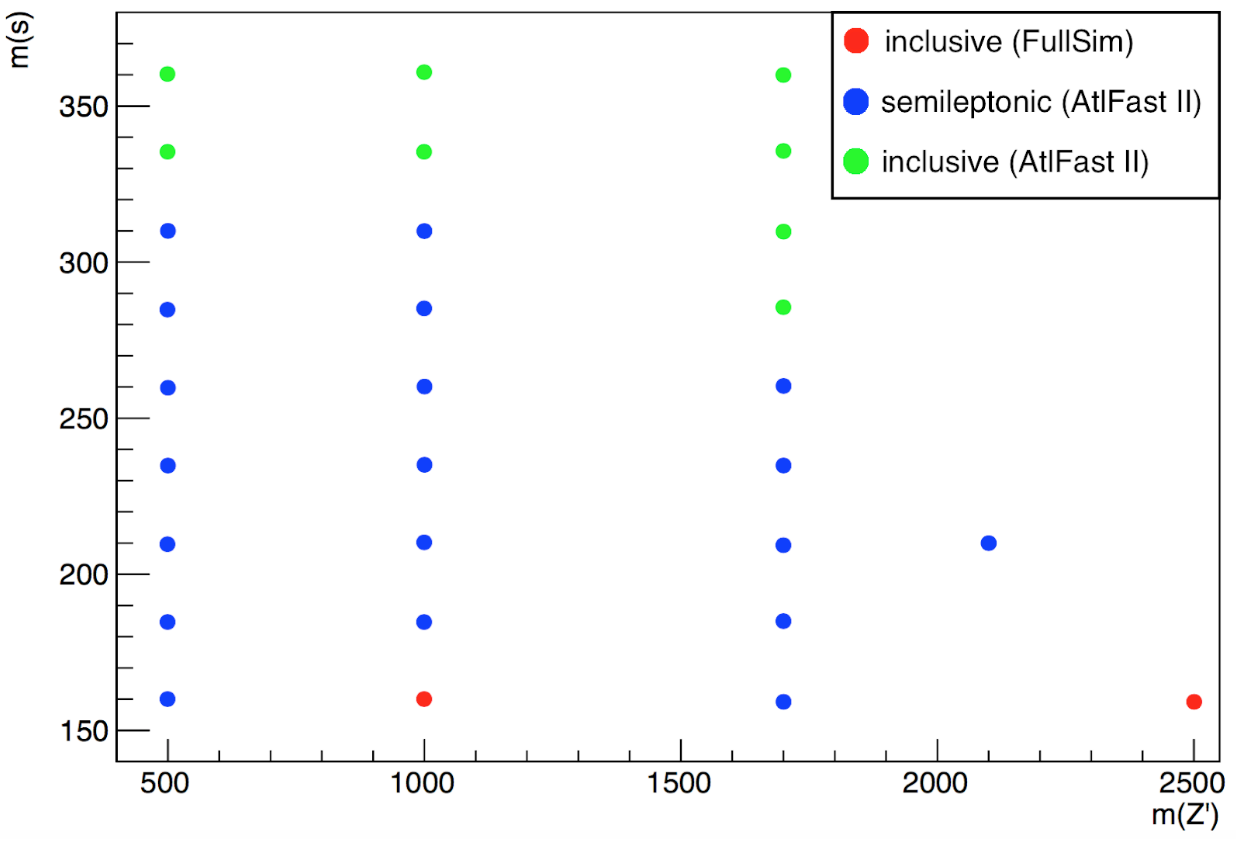
\includegraphics[width=0.7\textwidth]{figures/SignalGrid.png}
	\caption{Grid of signal points with respect to dark higgs (s) and Z' boson masses of generated signal sample}
	\label{fig:signalgrid}
\end{figure}

\begin{itemize}
	\item Scan over range of m(s) and m(Z')
	\item Need to fix some parameters in the model:
	\begin{itemize}
		\item $g_{q} = 0.25$
		\item $g_{\chi} = 1$
		\item $\theta = 0.01$
		\item $m_{\chi} = 200$ GeV
	\end{itemize}
	\item Discuss motivation for above choices of fixed model parameters
\end{itemize}

\section{Event Selection for Semileptonic Channel}

\subsection{Preselection}
\begin{itemize}
\item MET trigger passed
\item 1 signal lepton
\item MET > 150 GeV
\end{itemize}
\subsection{Regions}
\begin{itemize}
\item Signal region
\item W+jets control region
\item ttbar control region (if we plan to do one)
\end{itemize}
\subsection{Categories}
\begin{figure}[H]
     \centering
     \begin{subfigure}[b]{0.4\textwidth}
         \centering
         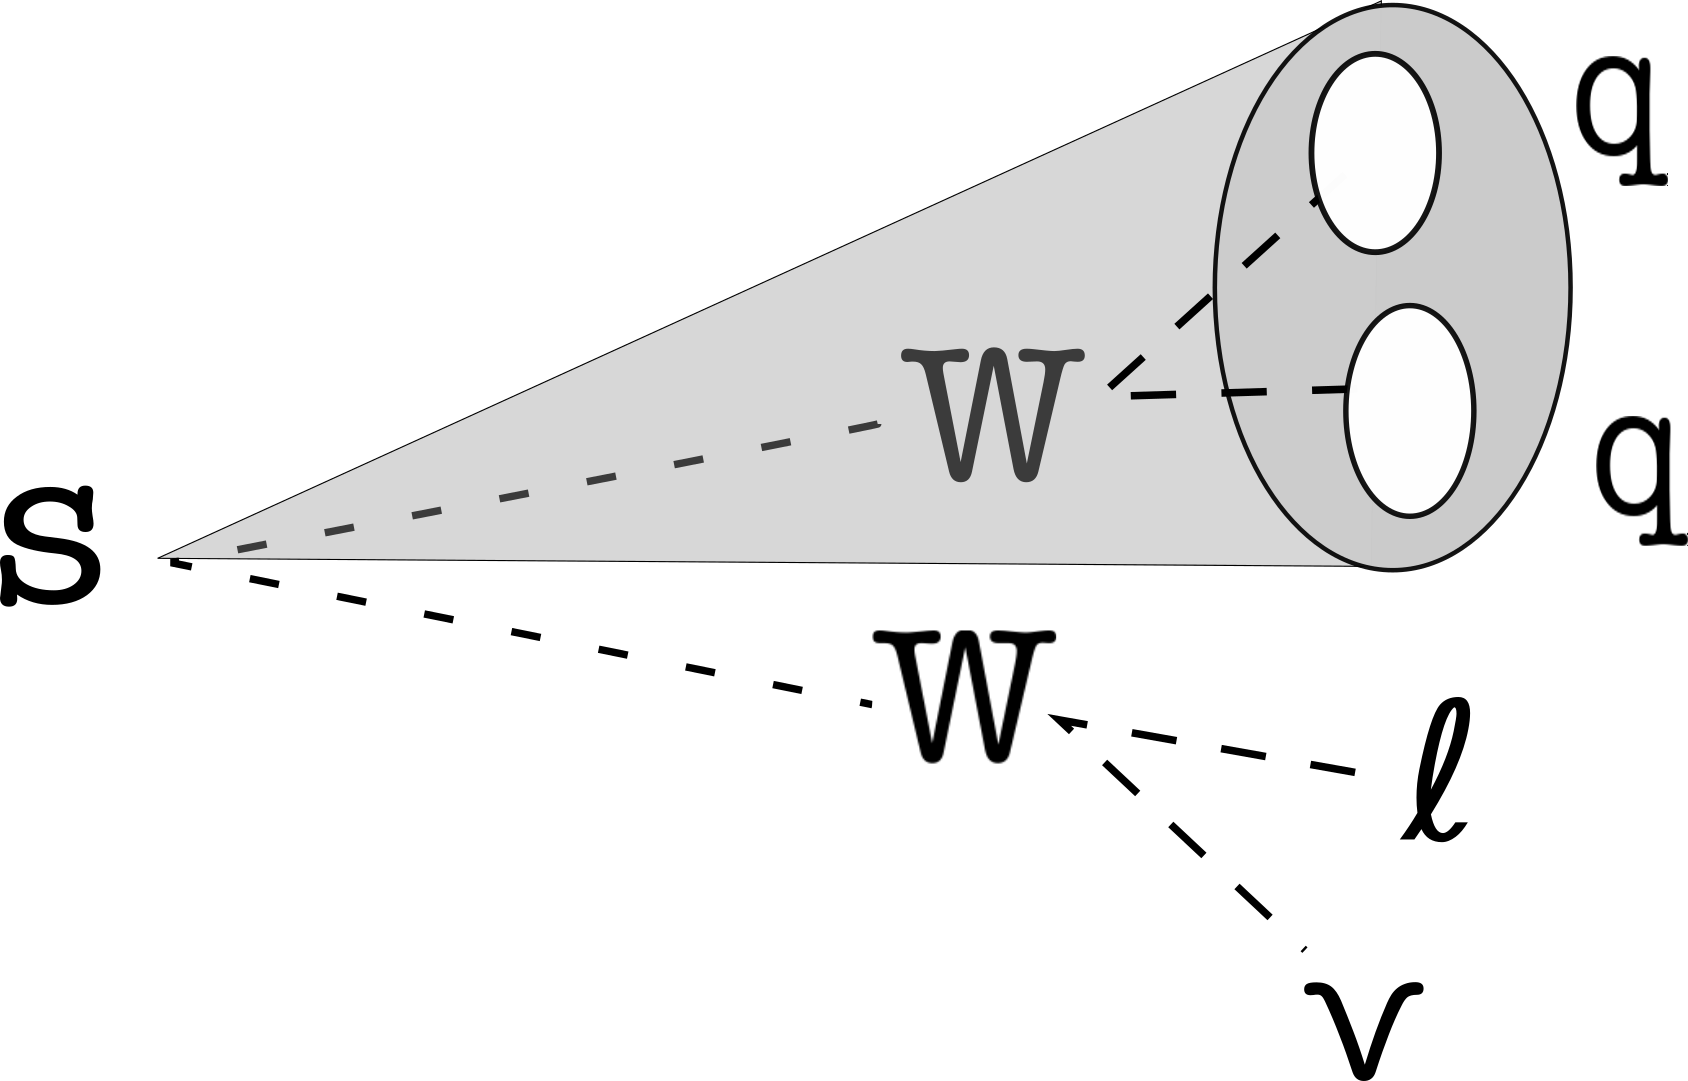
\includegraphics[width=0.9\textwidth]{figures/merged.png}
         \caption{Merged category}
         \label{fig:merged}
     \end{subfigure}
     \hfill
     \begin{subfigure}[b]{0.4\textwidth}
         \centering
         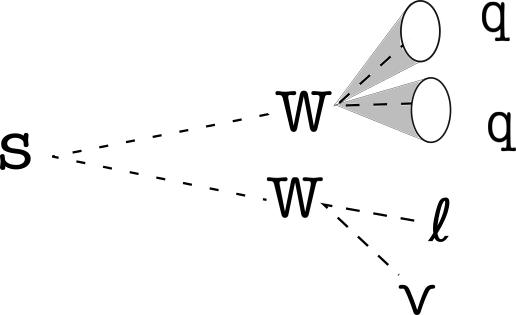
\includegraphics[width=0.9\textwidth]{figures/resolved.png}
         \caption{Resolved category}
         \label{fig:resolved}
     \end{subfigure}
\caption{Kinematic categories for final state selection}
\label{fig:categories}
\end{figure}
\begin{itemize}
\item Resolved category
\item Merged category
\end{itemize}


\section{Sensitivity Studies}
\subsection{Background on limit setting}
\subsection{HistFitter setup}
\begin{itemize}
\item Fit variable
\item Binning
\item Use of temporary systematics proxy
\end{itemize}
\subsection{Preliminary sensitivity limits}
\begin{itemize}
\item Resolved 
\item Merged 
\item Combined
\end{itemize}

\section{Remaining Work and Outlook}
\begin{itemize}
\item Study variables to help address $p_\nu$ vs. $p_{\chi\bar{\chi}}$ MET ambiguity
\item Finalize SR and CR definitions
\item Experimental and modeling systematics
\item Finalize sensitivity estimates with final systematics
\item Statistical combination with hadronic channel for combined limits
\end{itemize}

\bibliography{bibliography}
\bibliographystyle{plain}

\end{document}